\section{Introduction}
\label{intro}
Universities, knowledge centers and other institutions has the need for equipment that demonstrates physical phenomena in interesting and audience friendly ways. An example of this is a Double Resonant Solid State Tesla Coil (DRSSTC). This is a contraption that by the use of high voltage generates a sequence of electrical discharges. When these discharges happen in air a sound wave is generated. By modulating the frequencies of these discharges one can generate sound with different tones. A DRSSTC can in this way be made into a musical instrument.
For demonstration purposes it is important to control both streamer length and tone quality on such an musical instrument. It is further desirable that the instrument is portable, reliable, and safe to use.
In a portable DRSSTC consisting of several modules it is desirable to quickly detect if errors occurs, i.e. in the context of transport. With the base in an existing circuit design it should be designed a robust implementation with possibility to detect errors. It is further desirable to develop a rough understanding of how different design parameters affects the performance of an DRSSTC.

The system should take audio as input and output acoustic audio by means of an high voltage electric discharge in air creating plasma (streamer) by the means of a resonant transformer (tesla coil). The system should also be designed such that it will always be functional, and in the case of the system not being functional should fail in a safe and non-destructive way (safe having priority over non-destructive). As well as indicating witch part of the system is non-functional. The system should also be designed in such a way that this non-functioning part may be swapped for a spare functioning part.

\Cref{fig:teslabano} shows a DRSSTC in use where a streamer has formed from the top load to a grounded copper object.

\begin{figure}[ht]
    \centering
    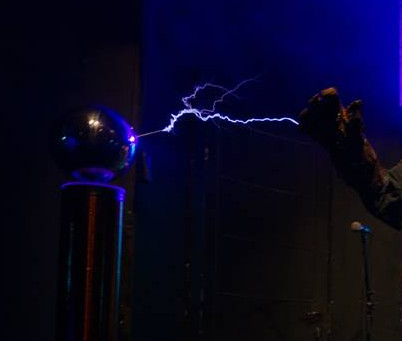
\includegraphics[width=0.6\textwidth]{img/teslabano.jpg}
    \caption{A tesla coil in use}
    Foto: Sindre Vaskinn Hunn
    \label{fig:teslabano}
\end{figure}

\subsection{Tesla}
\label{tesla}
%http://www.tfcbooks.com/tesla/contents.htm
The Tesla Coil is a form of resonant transformer invented by Nikolai Tesla and used for experiments with artificial illumination \citep{5570149}. A resonant transformer consists of two inductively coupled coils, each loaded with a capacitance such that they get the same resonance frequencies. The resonant transformer has since gotten a lot of applications, among others; RFID, NFC, and Wireless charging. The resonant transformer in the form of the Tesla Coil has also become a popular entertainment device.
%Death ray
%Entertainment